\chapter{主板及扩展板PCB设计}
\label{cha:PCB}

主板PCB设计如图:

\begin{figure}[htbp]
    \centering
    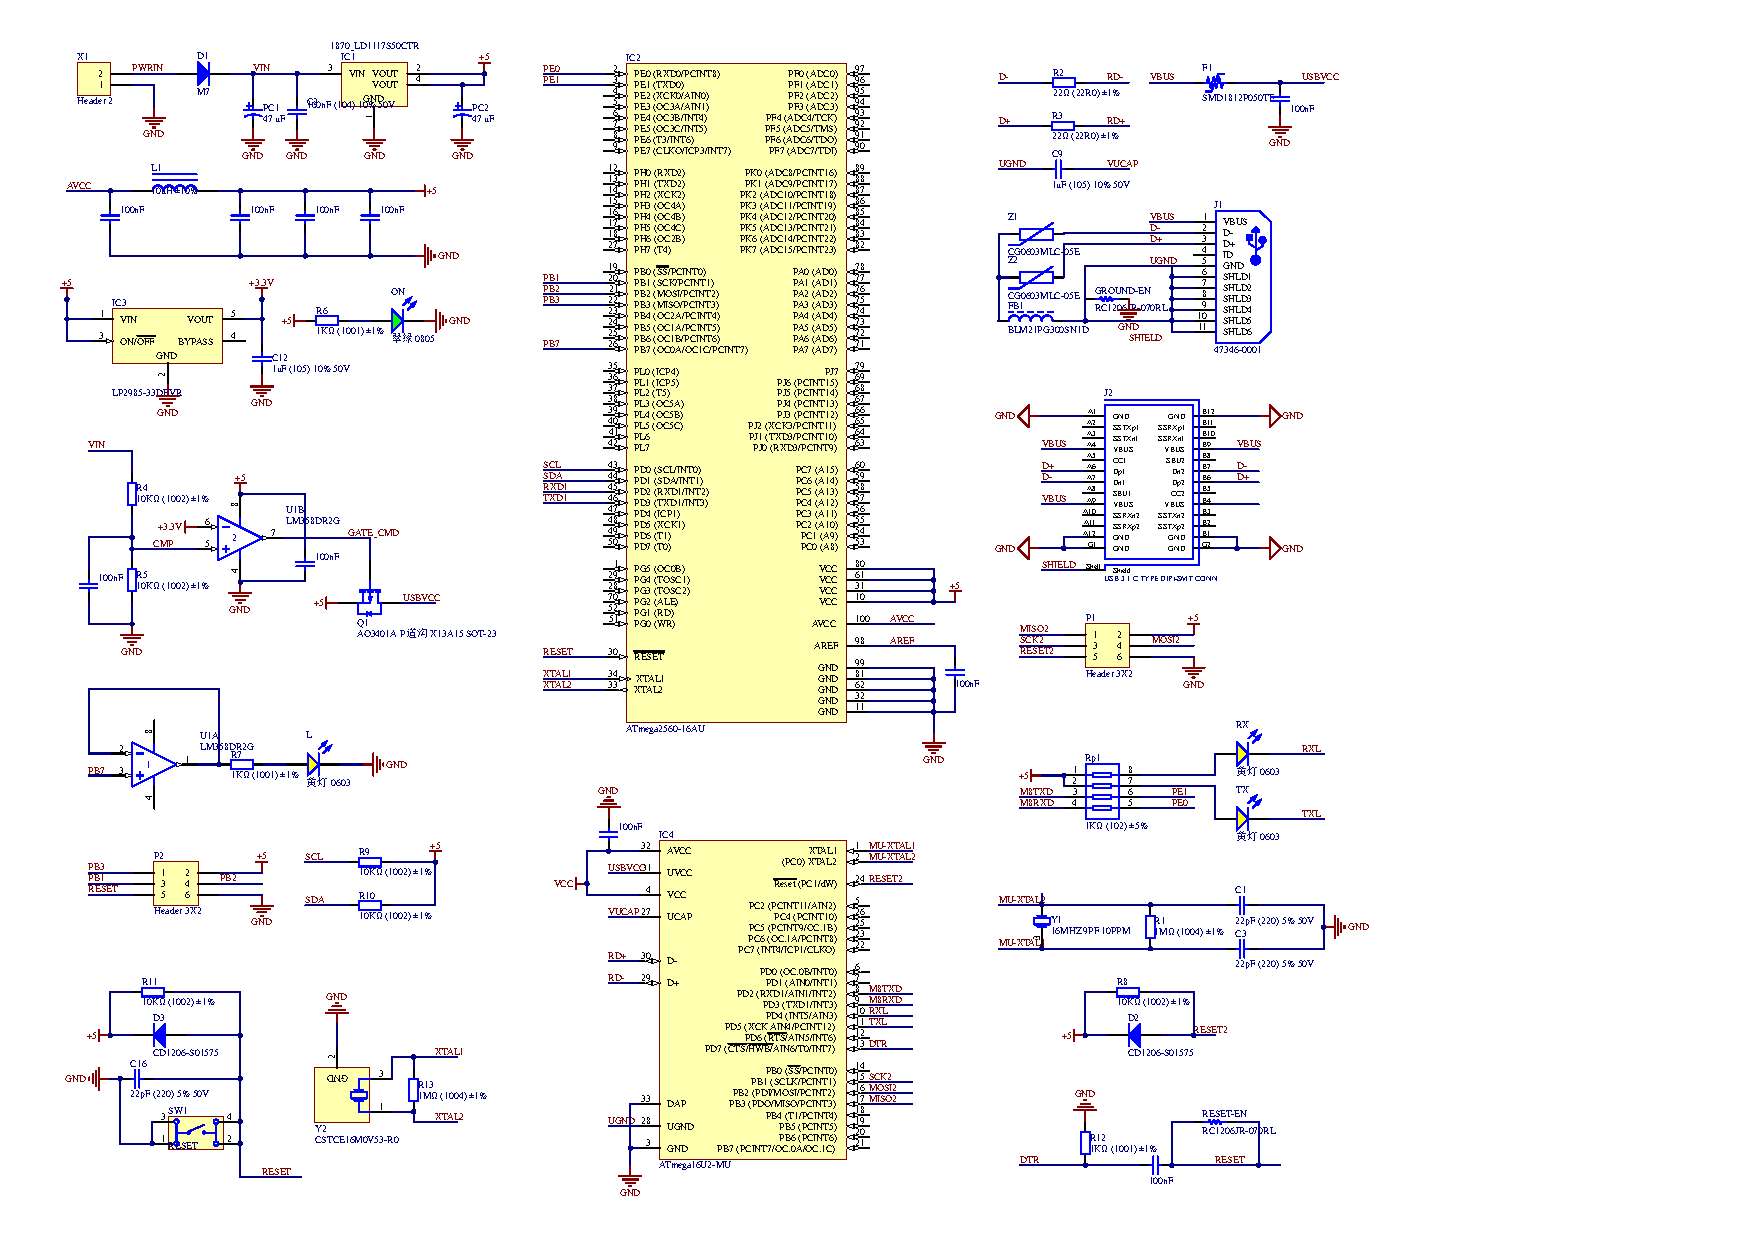
\includegraphics[]{ArduinoMega2560-Core-White-Crop.pdf}
    \caption{Mega 2560主板设计}
    \label{fig:CorePCB}
\end{figure}

\section{ATmega2560-16AU}

主控芯片拟采用ARDUINO MEGA 2560 REV3\cite{arduino_mega-2560-r3}上使用的ATmega2560-16U芯片\footnote{\href{http://www.atmel.com/Images/Atmel-2549-8-bit-AVR-Microcontroller-ATmega640-1280-1281-2560-2561_datasheet.pdf}{ATmega2560 Datasheet}},并参考MEGA 2560的芯片外设和烧写器设计。引脚映射图见附录~\ref{cha:Appendix-PCB}。

\begin{figure}[htbp]
    \centering
    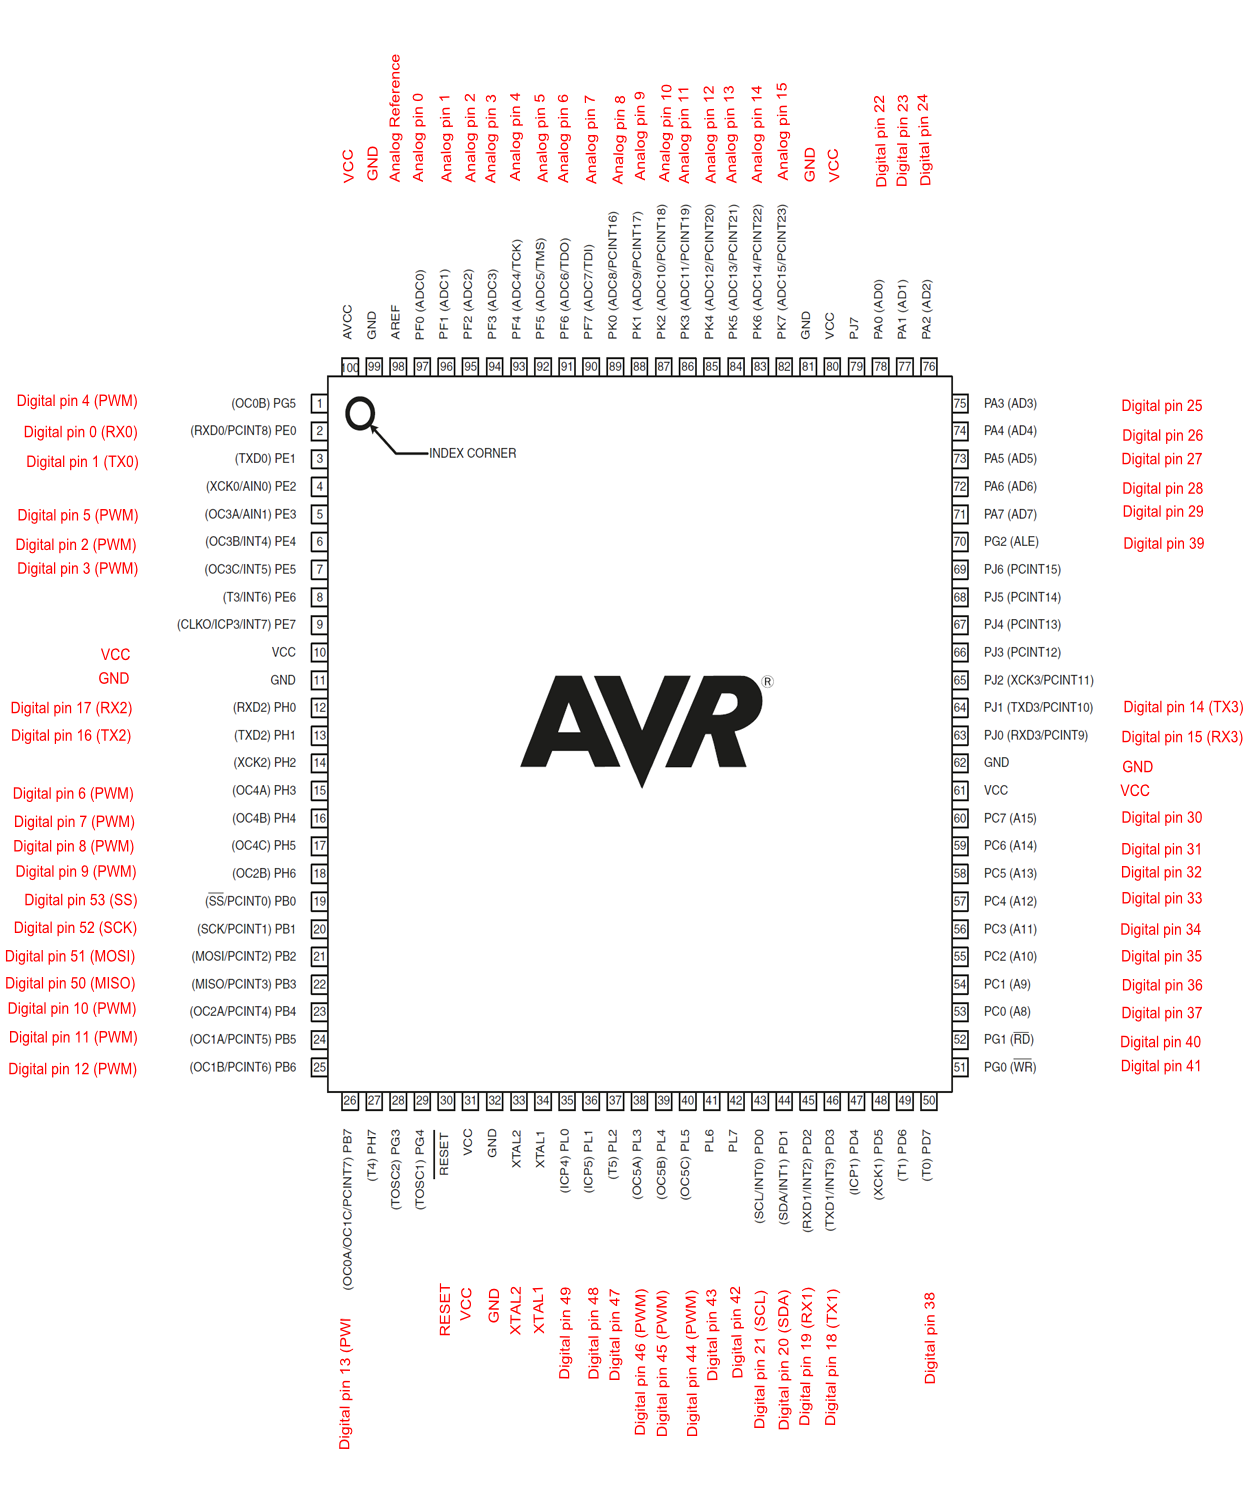
\includegraphics[width=0.7\textwidth]{PinMap2560big_Rev2.png}
    \caption{Mega 2560 PIN diagram}
    \label{fig:PinMap2560}
\end{figure}


\begin{figure}[htbp]
    \centering
    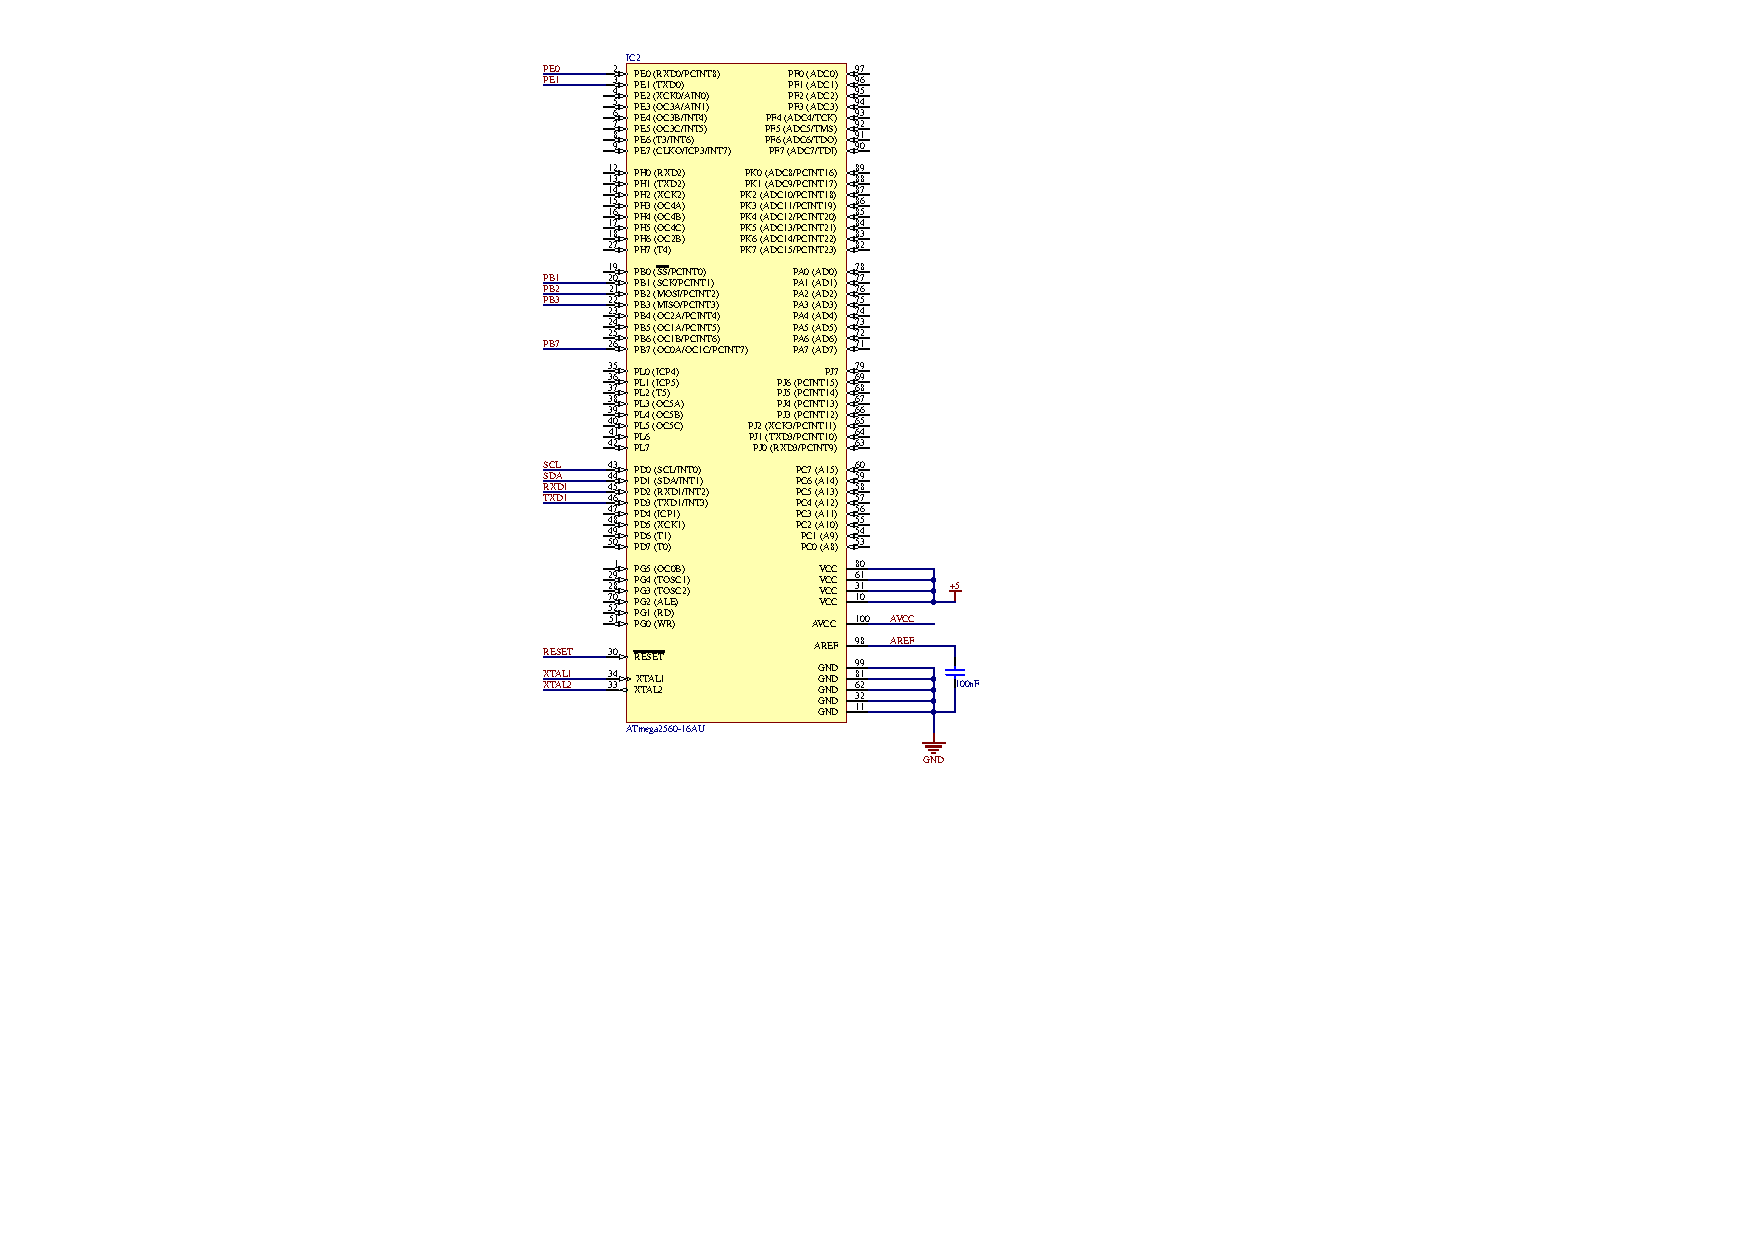
\includegraphics[]{Mega2560-ATmega2560-16AU.pdf}
    \caption{Mega 2560 MCU 原理图}
    \label{fig:Mega2560-ATmega2560-16AU}
\end{figure}

\section{扩展接口}

三明治扩展。

\section{接口}
为了紧跟潮流,我们使用USB Type-C接口进行供电和烧写程序:

\begin{figure}[htbp]
    \centering
    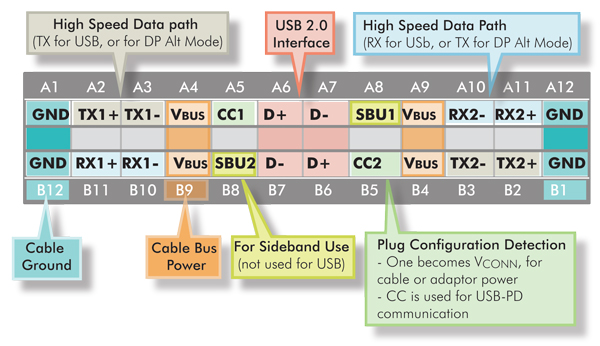
\includegraphics[width=\columnwidth]{Figure-2-USB-Type-C-pins.jpg}
    \caption{USB-Type-C-pins}
    \label{fig:USB-Type-C-pins}
\end{figure}

\begin{figure}[htbp]
    \centering
    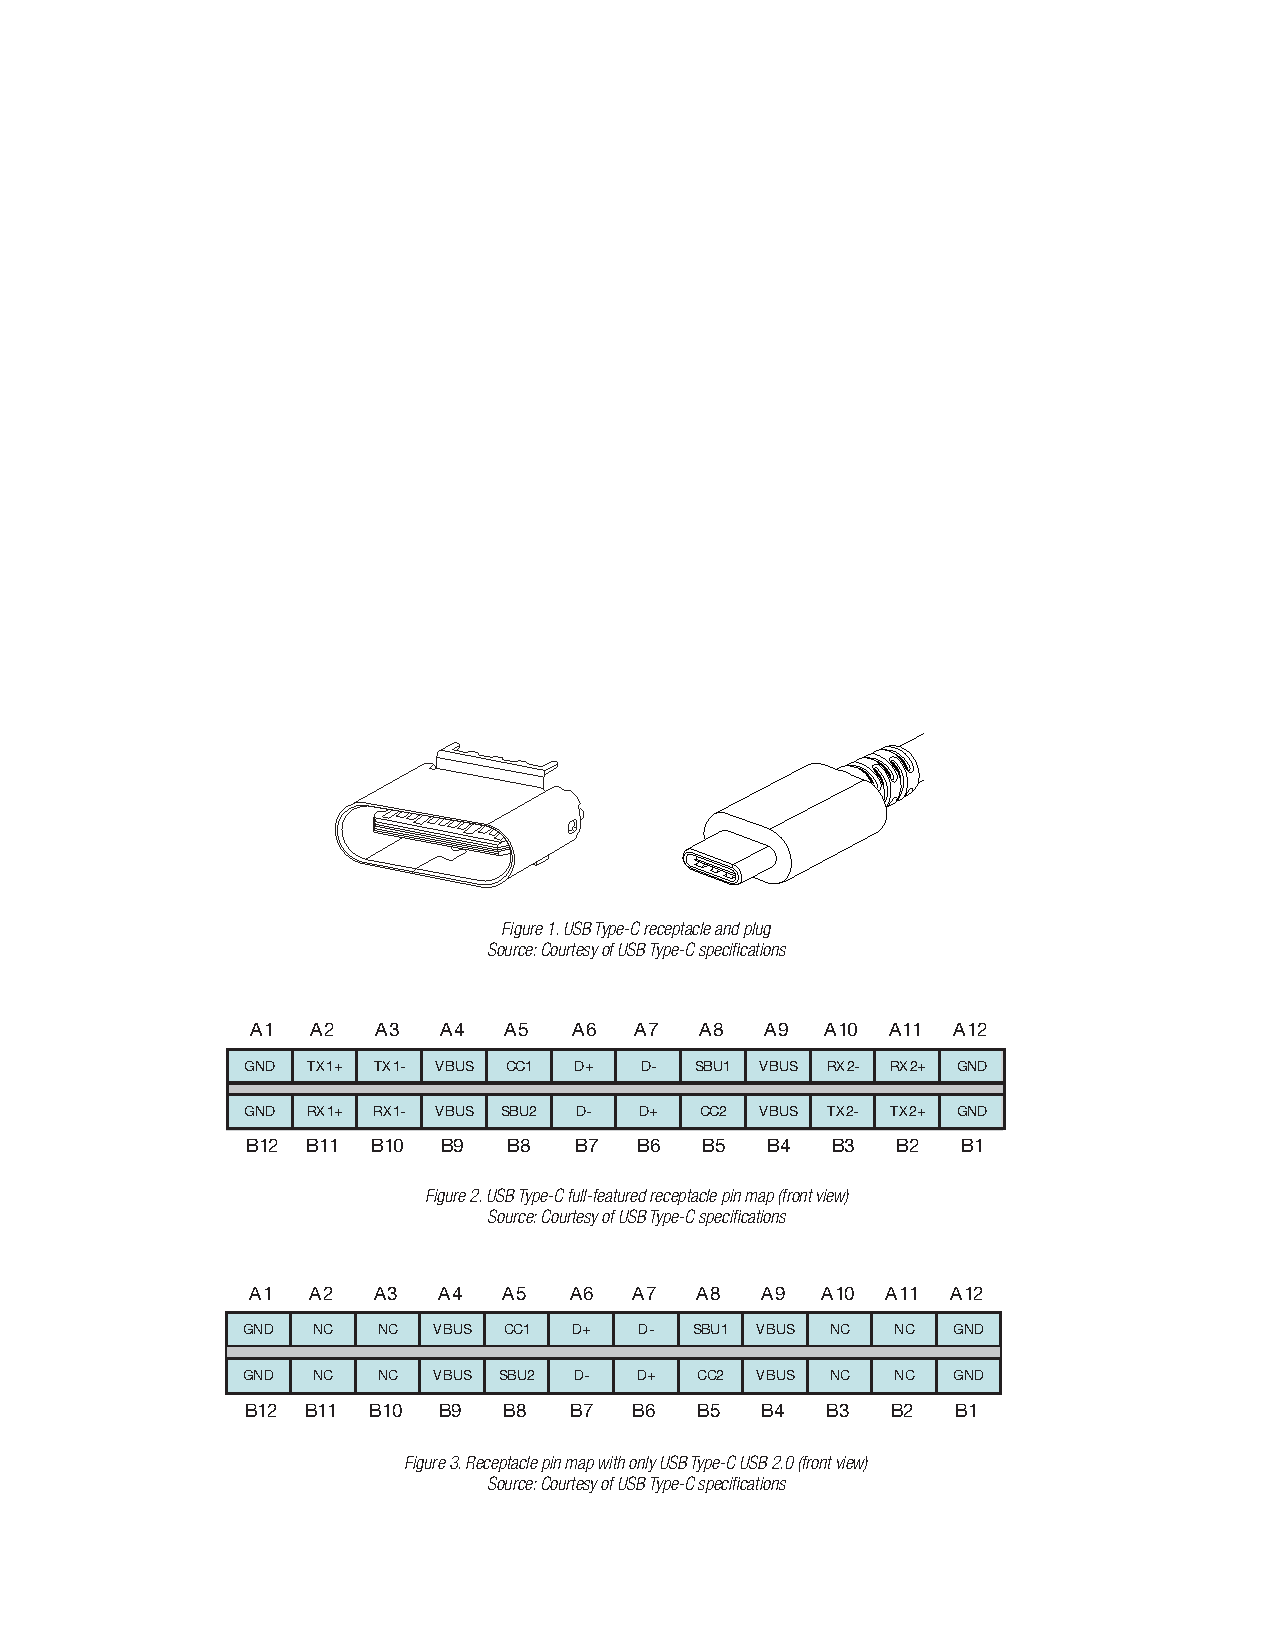
\includegraphics[width=\columnwidth]{USB-2-To-Type-C.pdf}
    \caption{USB-TypeC}
    \label{fig:USB-TypeC}
\end{figure}